\chapter{Patrones creacionales: Factoría Abstracta, Método Factoría y Prototipo}

\section{Caso de estudio: descripción en lenguaje natural}

A partir de nuestra aplicación, CaveArt, vamos a tomar el caso de la generación de entidades con distintas texturas alternativas.
Nos centraremos particularmente en la generación de animales.
Los animales de CaveArt tienen la particularidad de que, en función de algunos parámetros del juego, permite crear animales normales o sus versiones monstruosas, que son más grandes y hostiles (y visualmente más amenazantes).

En lugar de dejar la responsabilidad del tipo de animal a crear al \texttt{GestorEntidades}, la delegamos a una clase \texttt{AnimalFactory} usando el patrón \textbf{Factoría Abstracta}, de forma que sea ésta la que se encargue de decidir qué tipo de animal va a producir.
Al usar este método, facilitamos la creación de objetos evitando que el programador tenga que tener en cuenta diferentes tipos de constructores para los cientos de objetos que se pueden crear en el juego.

Dado que todos los animales son clases del mismo tipo, tiene sentido que todos sus constructores se implementen de la misma forma, por lo que usamos el patrón \textbf{Método Factoría} para unificar todos sus constructores, de forma que su acceso sea mucho más sencillo.
Al usar ese método, dejamos patente en el código que los objetos creados están estrechamente relacionados en su comportamiento y facilitamos la lectura del código.

Por último, nos interesa crear los animales a partir de una instancia del objeto con unos valores por defecto (por ejemplo, con el nivel de vida al máximo y el nivel de hambre al 75{\%}).
Para ello, usamos el patrón \textbf{Prototipo}, que nos permite construir los objetos clonando una instancia con los valores por defecto que nosotros decidamos.
Usando este patrón en lugar de llamar al constructor por defecto nos aseguramos de poder cambiar los atributos por defecto en tiempo de ejecución para ajustarlos a la situación actual del jugador

\pagebreak

\section{Aplicación de los patrones Factoría Abstracta y Método Factoría}

\begin{figure}[h!]
\begin{center}
	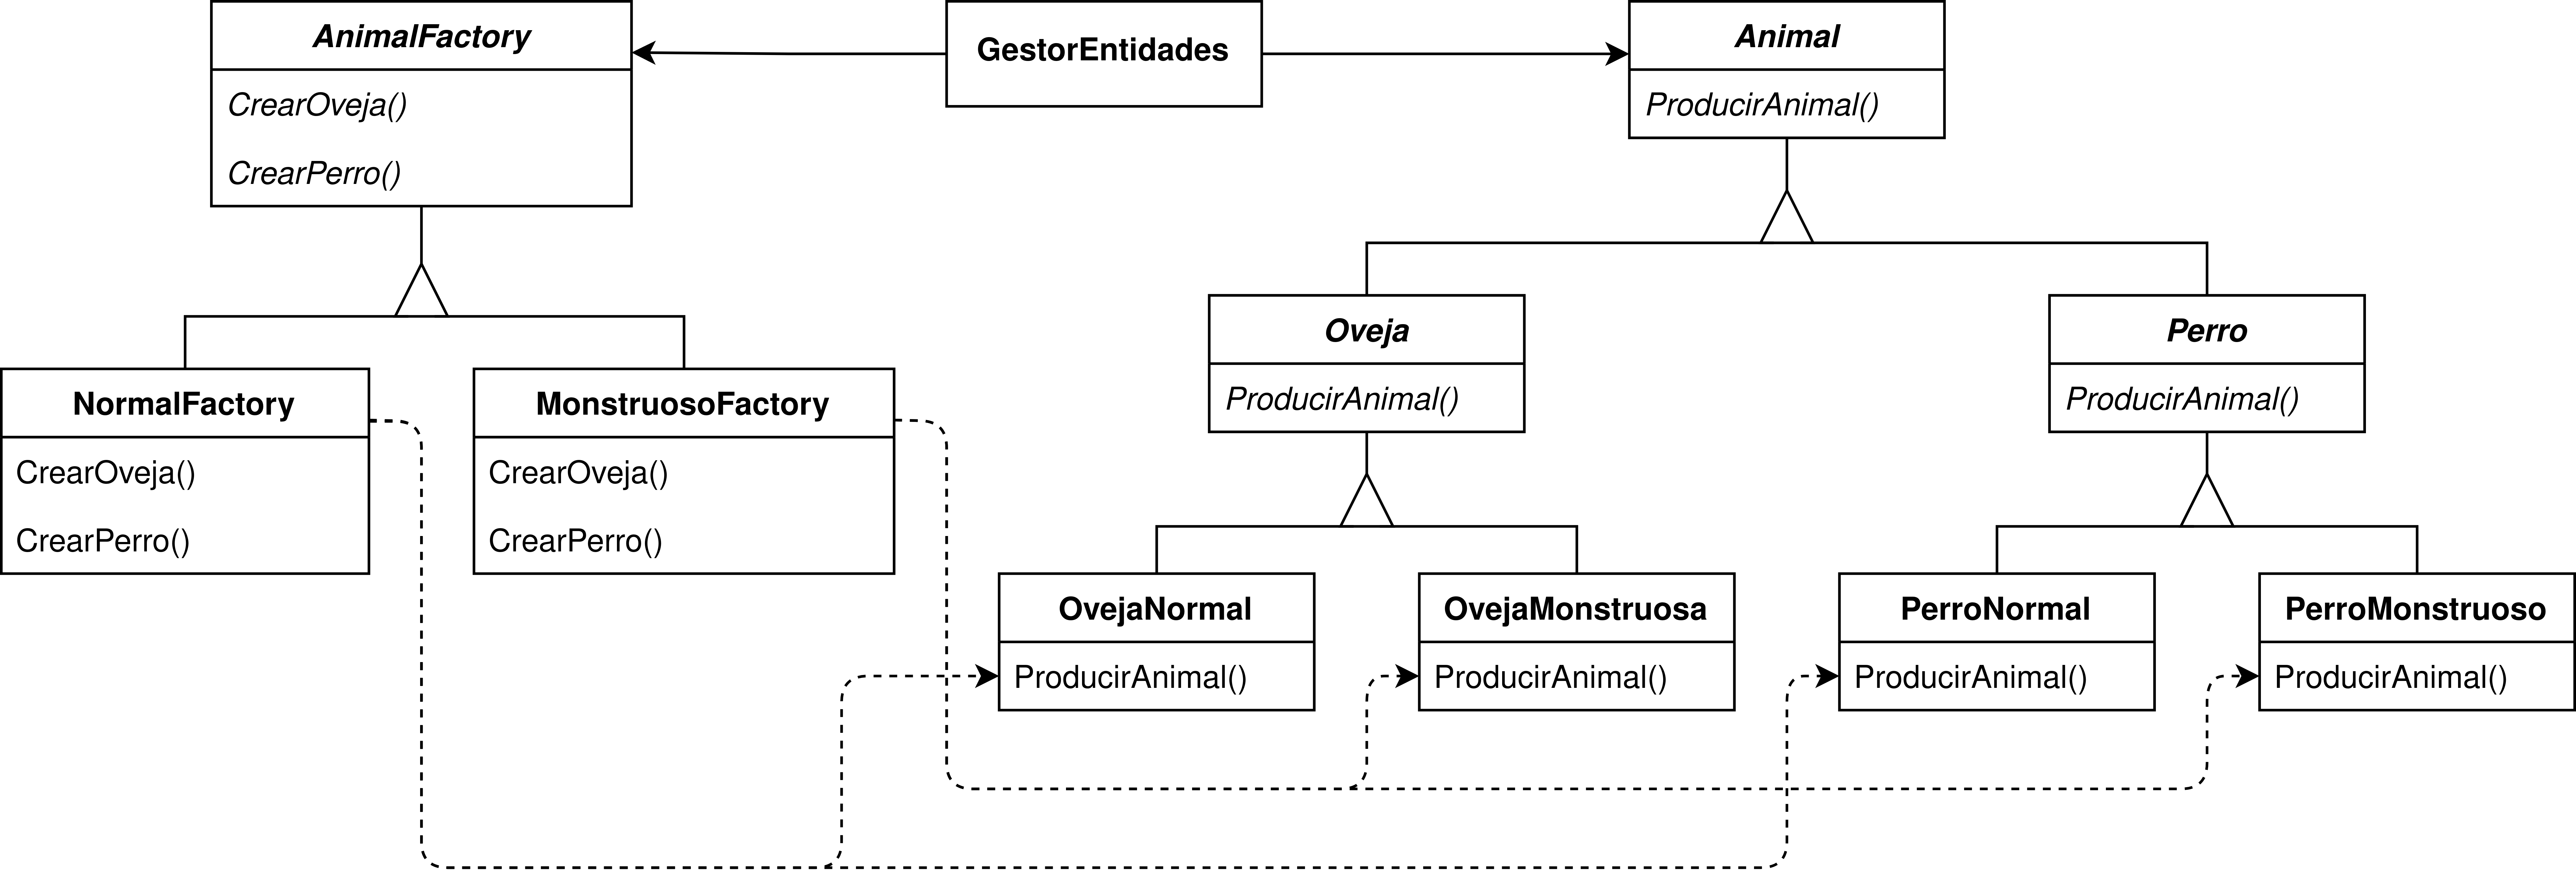
\includegraphics[scale=0.05]{Factoría Abstracta, Método Factoría.png}
\end{center}
\caption{Implementación de los patrones Factoría Abstracta y Método Factoría en CaveArt}
\end{figure}

\section{Aplicación de los patrones Factoría Abstracta y Prototipo}

\begin{figure}[h!]
\begin{center}
	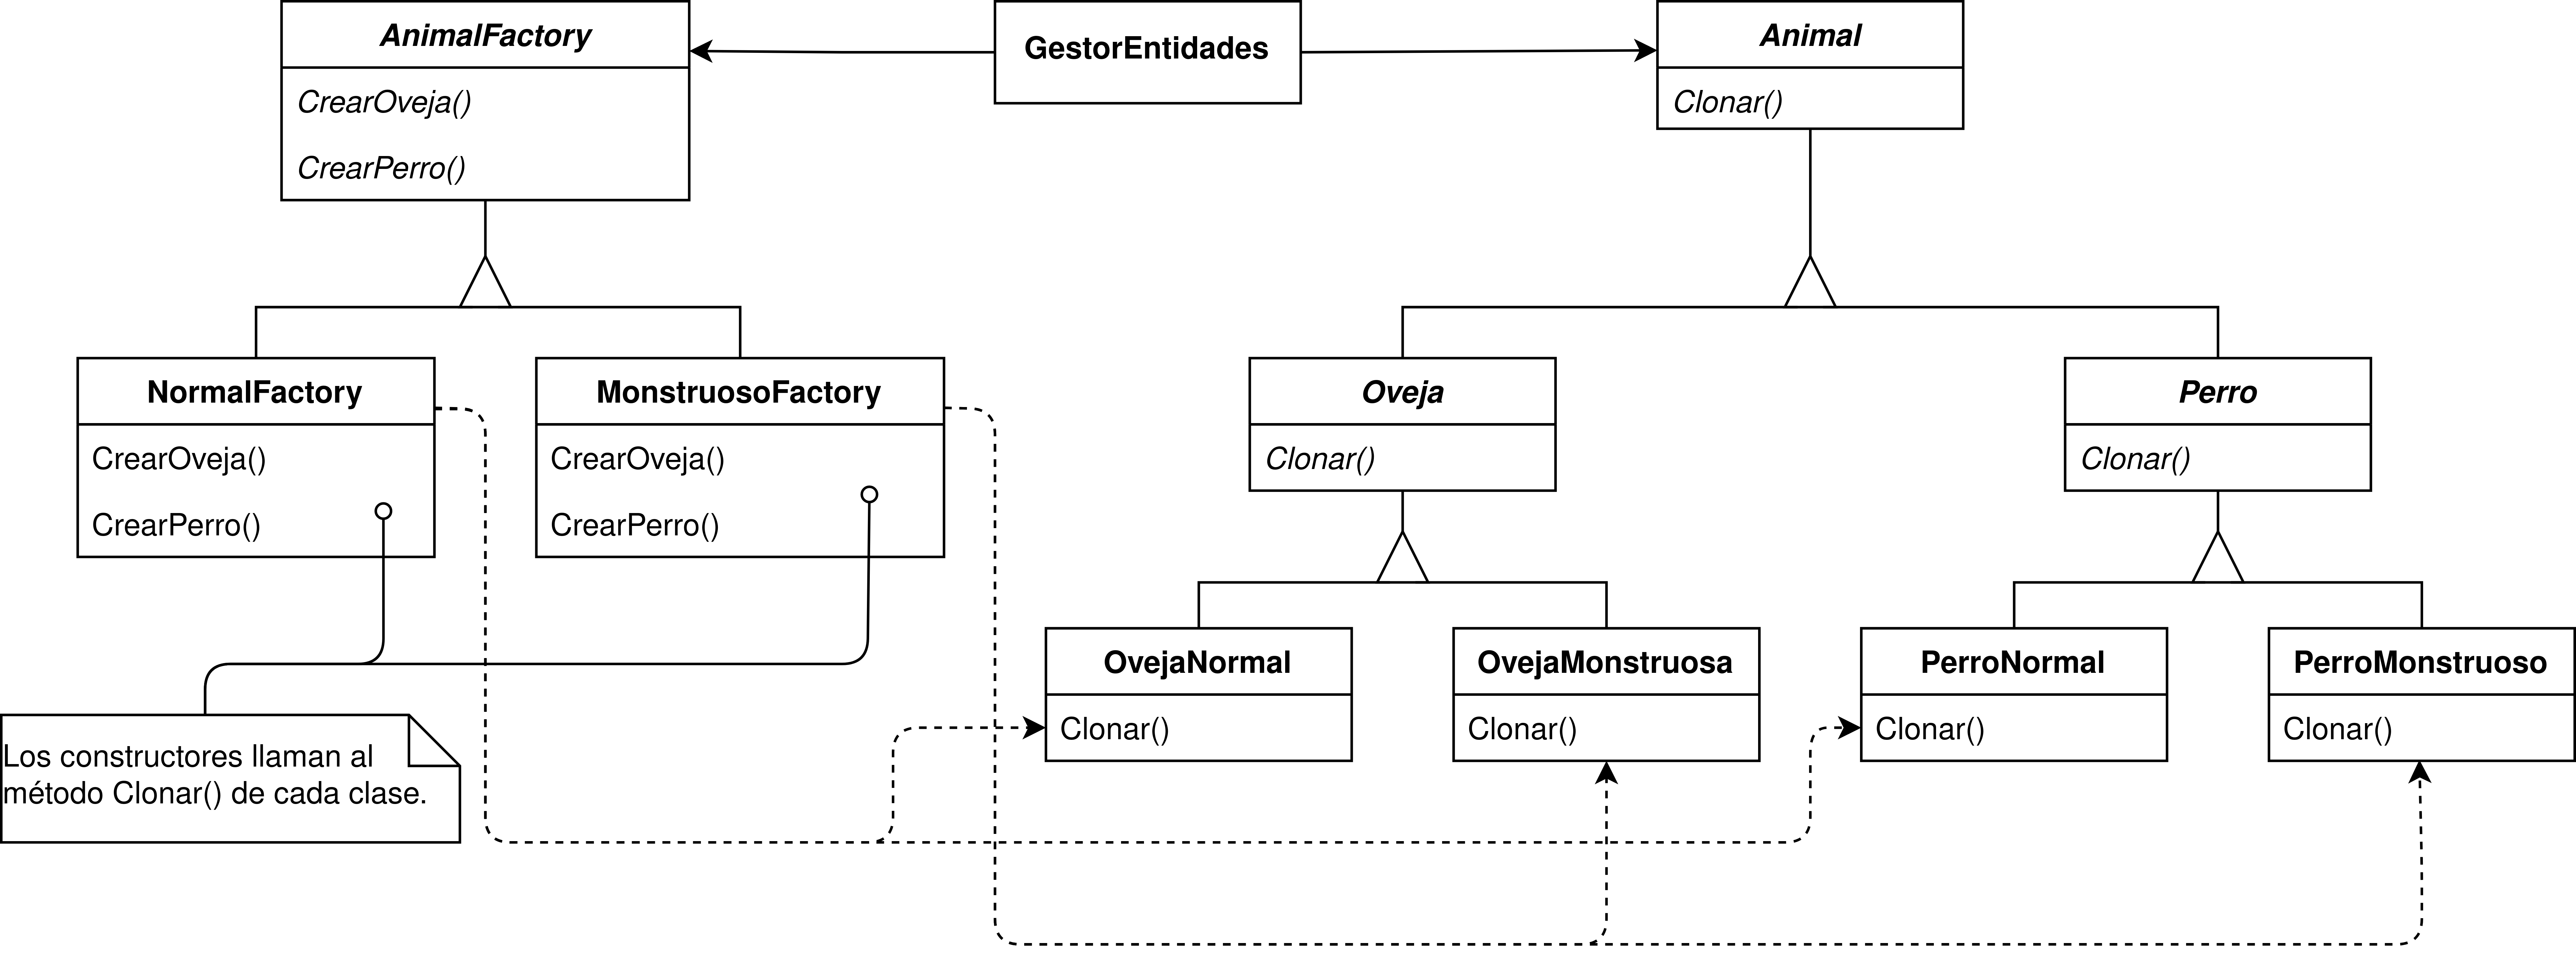
\includegraphics[scale=0.05]{Factoría Abstracta, Prototipo.png}
\end{center}
\caption{Implementación de los patrones Factoría Abstracta y Prototipo en CaveArt}
\end{figure}

